%! Author = vsharma
%! Date = 25.09.2022
% !TeX spellcheck = en_EN

\chapter{Related Work}

\section{Cloud Background}

\subsection{Cloud Computing}
Cloud computing in simple terms is defined as the delivery of computing services and resources. These include
storage, databases, servers, software, and networking over the internet. Cloud computing is a combination of two
words “cloud” which means “internet” and computing involves the systems and infrastructures that enable a computer to run and build, deploy, or interact with information. Cloud computing is a very common phrase that people hear nowadays but might not actually understand. It is because cloud computing encompasses several different services and systems thus making it ambiguous or confusing. In simple words, cloud computing can be defined as the delivery of computing services, these include databases, storage, servers, etc. over the internet \cite{11}.

Cloud computing enables the use of off-site systems which helps the computers to store, manage, process, and
communicate information. These services are available over the internet and are not hosted on-premises by the
organization. These systems can store anything from software programs to email servers, data storage, etc \cite{11}
\cite{12}.

\subsection{Types of cloud computing:}

\par There are different cloud providers that offer cloud services namely Amazon Web Services (AWS), the cloud computing service of Amazon.com, Microsoft Corporation’s cloud segment contains Azure, Google Cloud Platform (GCP), part of Alphabet Inc, etc. Each of the cloud platforms is unique in its own way and offers a plethora of options for organizations to select from based on their specific requirements. When considering the services offered by these clouds, AWS offers around 200+ services, whereas Azure offers up to 100+ services. Google Cloud, on the other hand, is catching up with Azure and AWS offering around 60+ services. In terms of the availability zones, AWS has 66 availability zones, Azure has 54 regions worldwide and is available in 140 countries all around the world, and Google Cloud Platform has been made available in 20 regions around the world \cite{13}. There are several factors to consider while deciding on a cloud service provider. In order to determine the most suitable type of cloud computing on which the cloud services can be implemented, it is better to first identify the type of cloud computing architecture or cloud deployment. There are three different cloud offerings to deploy cloud services: a private cloud, a public cloud, or a hybrid cloud \cite{14}.

\textbf{Private cloud:}
Private cloud refers to computing resources that are used by a particular organization or a single business.
In this,
the computing resources are owned, operated, and governed by the same organization.
In the private cloud, the cloud
computing resources are physically located at the organization’s on-site datacenter, the services and the
infrastructure are maintained by a private network \cite{14}.

\textbf{Public cloud:}
This type of cloud usually offers B2C (Business to Consumer) type of interactions. Public clouds are operated and
owned by a third-party cloud service provider which delivers these resources over the internet. AWS is an example of
a public cloud where the cloud service provider owns and manages all the software, hardware, and other supporting
services \cite{14}.

\textbf{Hybrid cloud:}
A hybrid cloud refers to the mixed storage, services, and computing environment comprises of a public cloud such as
AWS and an on-premises infrastructure, a private cloud. The hybrid cloud approach is the most widely used infrastructure configuration these days as it enables the organization
to continue using their on-premises servers while taking the advantage of available public cloud options like AWS,
and Azure. This enables the organization to comply with the data residency policies while leveraging the benefits and
security of the public cloud \cite{14}.


\subsection{Types of cloud services:}
\textbf{Infrastructure as a service (IaaS)}
\par Infrastructure as a service (IaaS) is a type of cloud computing service that offers essential storage, memory, compute, and related networking, such as
operating systems and databases, as a cloud service to replace the on-premises infrastructure. In a typical IaaS
architecture, the most essential components are hosted by the cloud providers such as Networking hardware, Servers, Storage, Physical hardware, etc. This feature enables IaaS to provide the same capabilities and technologies as offered by the traditional on-premises data centers \cite{9}. The customer needs to only perform a few steps:
\begin{itemize}
    \item Customers can access the services over the internet by logging in to the IaaS platform created by the cloud
    service provider \cite{15}.
\end{itemize}
\begin{itemize}
    \item Then the customer is required to create a Virtual Machine (VMs) on the cloud platform according to their
    requirements and then install the operating system (OS) on the VMs, deploy middleware, such as databases, create
    storage buckets for workloads and backups, and install the enterprise workload into that VM \cite{15}. This
    varies from service to service.
\end{itemize}
\begin{itemize}
    \item Finally, these VMs can be deployed along with databases, apps, desired tools, and the company’s workload \cite{15}.
\end{itemize}
IaaS benefits businesses by reducing operating costs, and by spending less on software upgrades and maintenance
\cite{15}.

\begin{figure}
    \centering
    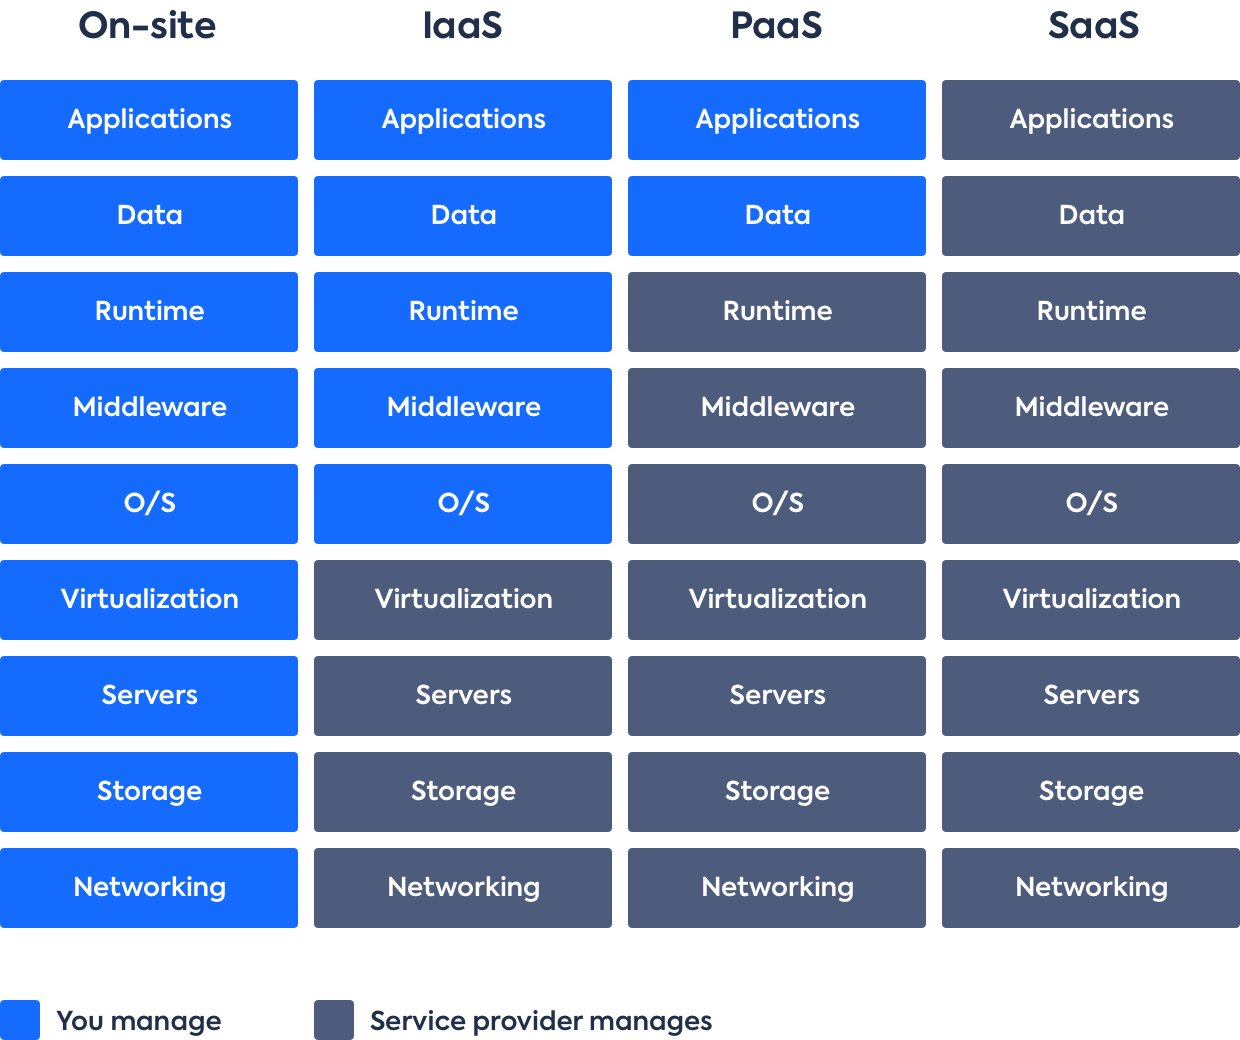
\includegraphics[width=\textwidth]{iaaspaassaas.jpg}
    \caption{Cloud computing models}
    \label{fig:iaaspaassaas}
\end{figure}

\textbf{Platform as a service (PaaS)}
\par PaaS is a cloud computing service that provides an on-demand environment for developing, testing, and managing software applications. PaaS is a cloud computing model that provides customers with a complete cloud platform—hardware, software, and infrastructure—for developing, running, and managing applications without the cost, inflexibility, and complexity that often come with building and maintaining that platform on-premises. It allows the developers to develop web and mobile applications without worrying about managing or setting up the underlying infrastructure for storage, servers, databases, and networks that are needed for deployment \cite{15}.

\par With PaaS, the organization avoids the complexity and expense of buying the software licenses, the underlying infrastructure, container orchestrators, development tools, and middleware or other resources. The organization only manages the application developed by them and cloud service providers such as Amazon AWS manage everything else \cite{9}.

\textbf{Software as a service (SaaS)}
\par Software-as-a-service (SaaS), also known as cloud application services, is the most comprehensive form of cloud computing services, delivering an entire application that is managed by a provider, via a web browser. Common examples are calendaring, email, and office tools (such as Microsoft Office 365). It is a distribution model in which the applications are hosted by cloud service providers or vendors to users across the globe. It is a software solution that can be purchased on a pay-as-you-go basis from a cloud service provider. In SaaS, all the application software, middleware, application data, and infrastructure are in the cloud service provider’s data center. The cloud service provider manages the software and hardware and ensures the security and availability of applications and data. It enables bringing up the organization’s application and running quickly and at a minimal upfront cost \cite{15}.

\par Figure \ref{fig:iaaspaassaas} describes the responsibilities of each deployment model compared to the on-premises setup.

\section{Amazon Web Services}
\par This section introduces the relevant AWS services and associated terminology used in this thesis. It is written to provide the reader with ample background knowledge required to understand this research work. It therefore by no means introduces the entire AWS platform.

\subsection{General AWS background}

\par Amazon web services is an evolving cloud computing subsidiary of Amazon. Amazon Web Services portfolio comprises more than 200+ services including database, compute, application development, security, infrastructure management, analytics, migration, etc. that help the organization to scale and grow. For example, AWS provides a wide range of databases that are designed specifically for specific applications. AWS  is a comprehensive, evolving cloud computing platform that includes a mixture of infrastructure as a service (IaaS), platform as a service (PaaS), and packaged software as a service (SaaS) offerings \cite{16}.
\par AWS was launched in 2006 and was one of the first cloud service providers to introduce a pay-as-you-go cloud computing model. It offers various tools and solutions for developers \cite{17}.

\par AWS cloud infrastructure is a highly secure, reliable, and extensive cloud platform \cite{18}. Whether it is required to deploy the application workloads globally with just one click, or to develop and deploy specific applications closer to the end user with latency in the single-digit millisecond range, AWS offers the right cloud infrastructure anywhere, anytime \cite{19}.

\begin{itemize}
    \item AWS Regions
    \item Availability zones
    \item Edge locations
\end{itemize}

\begin{figure}
    \centering
    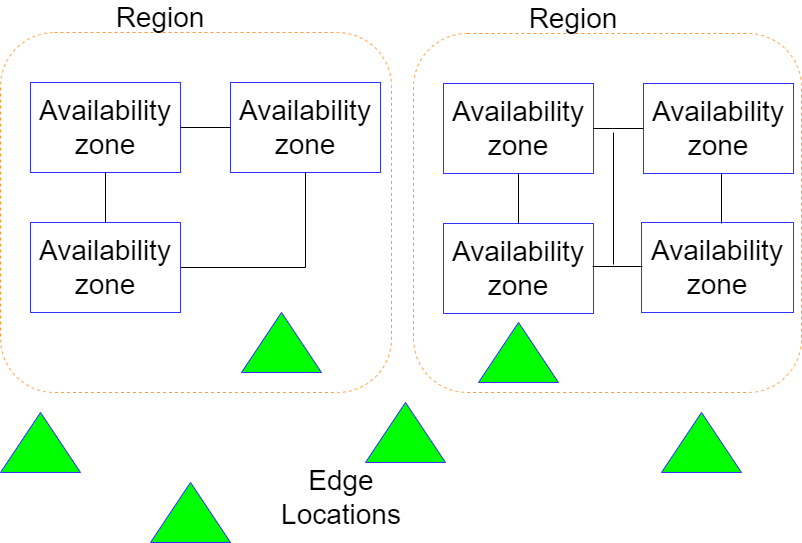
\includegraphics[width=\textwidth]{geographicalcomponents.png}
    \caption{AWS Geographical Components}
    \label{fig:identities}
\end{figure}

\par When designing and architecting the cloud infrastructure it is very important to know where the instances, services are data are located. This is a fundamental criterion to implement a highly available and scalable network that offers low latency \cite{19}.

\textbf{Region}
\par Regions are geographical locations to operate and run cloud services. These regions are spread globally and reduce the latency incurred by the customer when accessing the resource. Each AWS region contains availability zones. Within each of these regions, there are a minimum of 2 Availability Zones and a maximum of 6 Availability Zones, however typically 3 or more are usually found. The regions are connected to one another via a high-speed fiber network and are isolated from each other \cite{20}


\textbf{Availability zones}
\par Each region is made of a logical building block known as \textit{AWS Availability Zone (AZ)} and is isolated from the failures of other availability zones. The AWS regions operate independently and are isolated from other regions, but the availability zone within a region provides low-latency network connectivity to other Availability Zones within the same AWS Region. There is no explicit cost incurred for the network connectivity between two Availability Zones within the same AWS Region. Depending on the service used, in case of a failure, if an Availability Zone goes down, it is possible to ensure high availability by shifting the workload to another Availability Zone within the same region, this capability is known as \textit{Multi-AZ} redundancy. The figure \ref{fig:identities} shows 2 different AWS regions which are isolated from each other and each region consists of AWS Availability Zones \cite{21}.

\textbf{Edge Location}
\par In order to reduce the latency for the traffic, edge locations are deployed at multiple locations across the
world. Edge locations limit to building a new data center if the customers are in different cities or a different
part of the world. Edge locations can be understood as servers that are placed geographically close to the clients.
If we consider an example, an organization has many clients in Tokyo accessing the information which is deployed in a
region in Mumbai. In such cases, instead of clients sending requests constantly to Mumbai region for accessing the
information, we can cache a copy of the relevant information in Tokyo. Amazon CloudFront allows delivering video,
information, APIs to clients, or applications across the world. AWS CloudFront uses edge locations for accelerating
communication with customers \cite{22}.

\subsection{Services}

\textbf{AWS Identity and Access Management (IAM)}

\par Amazon Identity and Access Management (IAM) is a web service that helps to securely control access for the users to Amazon Web Services resources and services. Using IAM enables creating and managing Amazon Web Services groups and users and uses permissions to allow and deny their permissions to AWS resources. IAM enables organizations to create and control services for user authentication or limit access to a certain set of people who use their AWS resources \cite{23}.


\par IAM is a global service. When an AWS account is created, it begins with one sign-in identity. This identity has
complete access to all AWS resources and services in the account and is called the \textit{root user}. The AWS account root
user is accessed by signing in with the email address and password that you used to create the account. As
recommended, the usage of root users must be avoided for everyday tasks \cite{24}.

\begin{figure}
    \centering
    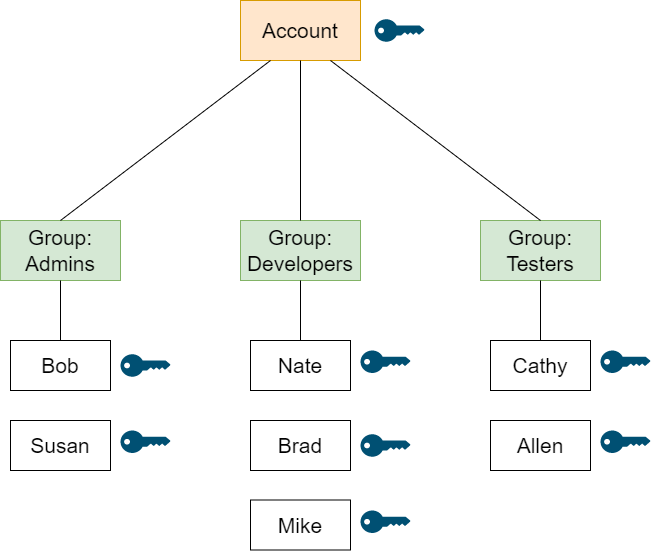
\includegraphics[width=\textwidth]{groupusers.png}
    \caption{IAM users and groups}
    \label{fig:groupusers}
\end{figure}

\textbf{IAM Users}

\par An IAM user is an identity within your AWS account that has specific permissions for a single person or application. Users have their own set of authentication parameters such as access key, secret key, or password that is required to access the AWS account through CLI or AWS console. An IAM user does not always represent an actual individual. Each IAM user is associated with only one AWS account \cite{25}.


\textbf{IAM Group}
\par An IAM group is an identity that specifies a collection of IAM users as show in the figure \ref{fig:groupusers}. The user
groups help in specifying the permissions for multiple users, thus making it easier to manage the permissions for the
users. For example, the organization could have a user group called Admins and give that user group typical
administrator permissions. Any user within a user group automatically has the permissions that are assigned to the
user group.
If a new user joins the organization and should have administrator privileges, the user can be assigned the
appropriate permissions by adding the user to that user group. Similarly, if a user changes a job role within the
organization, instead of editing that user's permissions, it is possible to simply remove them from the old user groups
and add them to the new user groups \cite{25}.



\textbf{Roles}
\par An IAM role is an identity within the AWS account that has specific permissions. An IAM role is similar to an IAM user but is not associated with a specific person. It is possible to temporarily assume an IAM role in the AWS Management Console by switching roles. Also, a role can be assumed by calling an AWS CLI or AWS API operation or by using a custom URL. However, a role is intended to be assumable by anyone who needs it instead of being uniquely associated with one person. Also, a role does not have standard long-term credentials such as access keys or passwords associated with it. Instead, when a role is assumed, it provides temporary security credentials for the role session. It is possible to use roles to delegate access to users, services, or applications that don't have access to your AWS resources. For example, it is required to grant users within an AWS account access to resources the users usually don’t have or grant users in one AWS account access to resources in another account \cite{25}.

\textbf{Policy}

\par An IAM policy is an IAM entity that sets permission and controls access to AWS resources. The IAM policies are
attached to AWS resources or IAM identities (users, groups, or roles) and define their permission. These policies are
evaluated when a principal such as a role or a user makes a request. Most policies in AWS are stored as JSON
documents. IAM policies define permissions which specify who has access to the resources and what operation they can
perform regardless of the method that is used to perform the operation. For example, if there exists a policy that allows the GetUser action, then a user with that policy can get user information from the AWS API or the AWS Management Console, or the AWS CLI. \cite{14}.

\par AWS provides six types of policies:

\begin{itemize}
    \item \textbf{Identity-based policies:} Identity-based policies are JSON documents that control what actions an
    identity
    (users, groups, and roles) can perform, under what conditions, and on which resources \cite{25}. The Identity-based policies can be further categorized as:
    \begin{itemize}
        \item Managed policies: Standalone identity-based policies that are attached to multiple users, groups, and
        roles in an AWS account \cite{25}.
    \end{itemize}
    \begin{itemize}
        \item Inline policies:  Policies that are added directly to a single identity such as user, group, or role.
        Inline policies maintain a strict one-to-one relationship between an identity and a policy and are deleted when the identity is deleted \cite{25}.
    \end{itemize}
\end{itemize}

\begin{itemize}
    \item \textbf{Resource-based policies:} Resource-based policies are JSON policy documents that are attached to a
    resource
    such as an Amazon S3 bucket. These are inline policies and grant the specified permission to perform specific actions on a resource \cite{25}.
\end{itemize}
\begin{itemize}
    \item \textbf{IAM permissions boundaries:} A permissions boundary is used to set the maximum permissions that an
    identity-based policy can grant to an IAM entity. When the permissions boundary for an entity is set, the entity can perform only the actions that are allowed by both its permissions boundaries and its identity-based policies. Resource-based policies that specify the user or role as the principal are not limited by the permissions boundary \cite{25}.
\end{itemize}
\begin{itemize}
    \item \textbf{Organizations Service control policies (SCPs):} Amazon Organizations is a service for grouping and centrally managing the Amazon accounts that the business owns. It helps to centrally manage and govern the environment as the organization grows and scales its AWS resources. Amazon Organizations is used to define the maximum permissions for account members of an organization or organizational unit (OU). AWS Organizations service control policy (SCP) limits permissions that identity-based policies or resource-based policies grant to entities (users or roles) within the account, but do not grant permissions \cite{25}.
\end{itemize}
\begin{itemize}
    \item \textbf{Access control lists (ACLs):} ACLs is used to control which principals in other accounts can access
    the
    resource to which the ACL is attached. ACLs are like resource-based policies, although they are the only policy type that does not use the JSON policy document structure. ACLs are cross-account permissions policies that grant permissions to the specified principal. ACLs cannot grant permissions to entities within the same account \cite{25}.
\end{itemize}
\begin{itemize}
    \item \textbf{Session policies:} Session policies are advanced policies that are passed as a parameter for
    programmatically creating a temporary session for a role or federated user. The permissions for a session are the intersection of the identity-based policies for the IAM entity (user or role) used to create the session and the session policies \cite{25}.
\end{itemize}

Figure \ref{fig:iamidentities} shows the overview of AWS IAM concepts in AWS infrastructure.


\begin{figure}
    \centering
    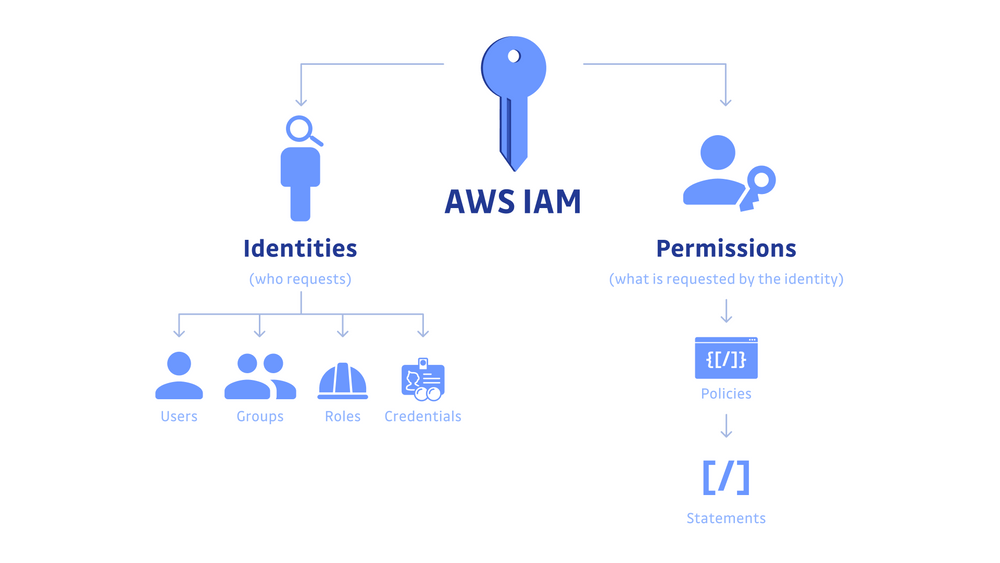
\includegraphics[width=\textwidth]{iaminfrastructure.png}
    \caption{Overview of AWS IAM concepts}
    \label{fig:iamidentities}
\end{figure}



\textbf{Features of IAM}

\begin{itemize}
    \item \textbf{Granular permissions:} Based on the usage, permissions can be granted to different people to access
    different resources. For example, some users are granted complete access to Amazon Simple Storage Service (Amazon
    S3), Amazon Elastic Compute Cloud (Amazon EC2), Amazon DynamoDB, and other AWS services while other users are only
    provide permissions to administer some EC2 instances, read-only access to some S3 buckets but no other services \cite{25}.
\end{itemize}
\begin{itemize}
    \item \textbf{Multi-factor authentication (MFA):} To enable enhanced security of the AWS account, it is possible
    to enable
    two-factor authentication to the root account as well as to the individual users’ account. This ensures the AWS user along with providing the username and password for the account also provides a code from a configured device \cite{25}.
\end{itemize}
\begin{itemize}
    \item \textbf{Identity federation:} Identity federation is a system of trust between two parties for the purpose of authenticating users and conveying the information needed to authorize their access to resources. Identity federation allows users to log in to the AWS console who have their password in the Active directory or elsewhere such as in the internet identity provider or in the organization's corporate network. An Active Directory uses a structured data store as the basis for a logical, hierarchical organization of directory information. It provides methods for storing directory data and making this data available to network users and administrators. For example, active directory stores information about user accounts, such as names, passwords, phone numbers, and so on, and enables other authorized users on the same network to access this information \cite{26}. For example, if a user has logged in to his Google account and would like to use the AWS account, then identity federation helps AWS IAM to trust the authentication method. This authentication enables temporary access to the user’s AWS account \cite{25}.
\end{itemize}
\begin{itemize}
    \item \textbf{Password policy:} Password is used to authenticate a user’s account and a strict password policy
    can make it
    even more secure. IAM password policy allows for password rotation and resetting the password remotely. It is
    possible to set rules such as a password must contain a number, special characters, or special symbols \cite{25}.
\end{itemize}


\textbf{Amazon Elastic Compute Cloud (EC2)}

\par Amazon elastic Compute cloud EC2 is one of the core services offered by AWS which provides scalable computing
capacity in the Amazon Web Services (AWS) Cloud. Amazon EC2 avoids upfront hardware setup investment, enabling faster
development and deployment of applications. Amazon EC2 enables launching as few or as many virtual servers as needed,
managing storage, and configuring security and networking. With Amazon EC2 it is possible to scale up or down to
handle changes in requirements or reduce the need to forecast traffic, and spikes in popularity \cite{27}.

\par Amazon EC2 offers a virtual computing environment called \textit{instances} which comes in different configurations of CPU, memory, storage, and networking resources to suit user needs. EC2 instances can be used for any computing task, for example as a web server. An AWS user can create, launch, and terminate an instance based on the need, paying by the second for active servers and hence the term elastic. Amazon EC2 provides users with control over the geographical location of instances that allows for latency optimization and high levels of redundancy. Placing all of the instances into the same AZ will likely give us the best latency between them. When an EC2 instance is provisioned, by default each instance is assigned automatically a DNS name and a public and private IPV4 address \cite{28}.

\textbf{Features of EC2}
\begin{itemize}
    \item \textbf{Elastic Web-Scale Computing:} Amazon EC2 enables users to expand the capacity as per their needs within the minutes, not hours or days. It is possible for the user to commission one, hundreds, or even thousands of server instances simultaneously. Many servers can be run in parallel with these instances. These services give the user a choice to increase or decrease the automation as per their needs \cite{29}.
\end{itemize}

\begin{itemize}
    \item \textbf{Versatile cloud hosting services:} Amazon EC2 gives users the choice to select from a variety of instance types, operating systems, and software packages. Amazon EC2 allows selecting a configuration of memory, instance storage, CPU, and boot partition size that is optimal for your choice of operating system and application. For example, the operating system options include a variety of Linux variants as well as Microsoft Windows Server \cite{29}.
\end{itemize}

\begin{itemize}
    \item \textbf{Security:} Cloud security is the highest priority at AWS. Amazon works with the Amazon VPC to provide additional security, isolating resources, and robust networking for the compute resources. The compute instances in AWS are located in the VPC in the specific IP range. Further, the user decides which instances are exposed to the internet and which remain private \cite{29}.
\end{itemize}

\begin{itemize}
    \item \textbf{Intended for use in conjunction with other Amazon web services:} Amazon EC2 collaborates with most
    AWS services such as Amazon Relational Database Service (Amazon RDS), Amazon Virtual Private Cloud (Amazon VPC), Amazon Simple Queue Service (Amazon SQS), and Amazon Simple Storage Service (Amazon S3) to provide a complete, secure, comprehensive solution for computation, query processing, and cloud storage across a wide range of applications \cite{29}.
\end{itemize}

\begin{itemize}
    \item \textbf{Completely controlled:} Users have complete control over the instances including root access and the ability to interact with instances just like any other system. Users can stop the instance while keeping the data on the boot partition, and then restart it using web service APIs. Using web service APIs makes it possible to reboot the instances remotely \cite{29}.
\end{itemize}

\textbf{Amazon Machine Image (AMI)}

\par An Amazon Machine Image (AMI) is a maintained and supported image provided by AWS. An AMI provides the necessary information required for launching an instance. An AMI must be specified while launching an instance. It is possible to launch multiple instances of the same configuration from a single AMI. When instances of different configurations need to be launched, different AMI must be used \cite{30}.

\begin{figure}
    \centering
    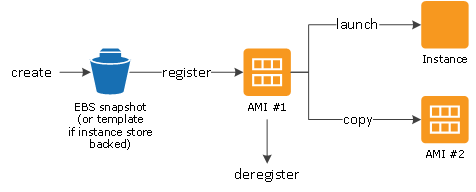
\includegraphics[width=\textwidth]{ami.png}
    \caption{Amazon Machine Image}
    \label{fig:ami}
\end{figure}

\par An AMI includes \cite{30}:
\begin{itemize}
    \item One or more Amazon EBS (Amazon Elastic Block Store) snapshots, or, for instance-store-backed AMIs, a template for the root volume of the instance (for example, an application server, an operating system, and applications).
\end{itemize}
\begin{itemize}
    \item Launch permissions that control which AWS accounts can use the AMI to launch instances.
\end{itemize}
\begin{itemize}
    \item A block device mapping that specifies the volumes to attach to the instance when it's launched.
\end{itemize}



\par Figure \ref{fig:ami} shows the lifecycle of AMI. Once the Amazon Machine Image (AMI) is created, it is stored in
an Amazon S3 bucket. This image is then registered and can then be used to launch a new instance. An AMI can be
copied to the same as well as to different AWS regions. If the AMI is not required any longer, it can be deregistered. Once deregistered the AMI cannot be used to launch new instances, but the existing instances using AMI will not be affected \cite{30}.

\par It is possible to launch an instance using an existing AMI. If the instance is customized, for example, the
software is installed on the image, this customized AMI can be saved with the updated configuration. Launching an
instance from this customized image contains customizations that were made earlier. To restrict the availability of
an AMI it can be made private, alternatively, the AMI is made public when the access doesn’t need to be restricted \cite{31}.




\textbf{Instance metadata and user data}
\par Instance metadata is the data associated with your EC2 instance that can be used to manage or configure the
running instance using the Instance metadata service (IMDS). Each EC2 instance has access to the Instance metadata
service (IMDS). The instance metadata is divided into different categories such as events, hostnames, and security
groups. Instance metadata service contains information about the running EC2 instance and can be used to capture the temporary API credentials for accessing the AWS APIs \cite{32}.

\par Instance metadata can be used to access user data that is specified when launching the instance. For example, it
is possible to specify parameters for configuring the instance or include a simple script. It is also possible to
build generic AMIs and use user data to modify the configuration files supplied at launch time. When more than one instance is launched at the same time, the user data is available to all instances. Each instance has a unique number called the ami-launch-index number. This number allows for writing code that controls what to do. For example, the first host might elect itself as the original node in a cluster \cite{33}.

\textbf{Amazon Relational Database Service (RDS)}

\par Amazon Relational Database Service (RDS) is a set of managed services that make it easy to set up, operate, and scale databases in the Amazon Web Services Cloud. Amazon RDS supports an array of database engines to organize and store data. It also helps with relational database management tasks, such as data backup, patching, recovery and migration. Amazon RDS provides its users access to the functionality of a familiar MariaDB, MySQL, SQL Server, Oracle, or PostgreSQL database. It facilitates the deployment and maintenance of relational databases in the cloud. The figure \ref{fig:rds} shows the different database services offered by Amazon RDS. Amazon RDS manages common database administration tasks and provides cost-efficient, resizable capacity for an industry-standard relational database. It provides an opportunity to choose an instance type for various database use cases. The database instance varies with respect to the memory, CPU, network capacity, and storage, thus providing flexibility in choosing the ideal combination of resources for your database \cite{34}.
\begin{figure}
    \centering
    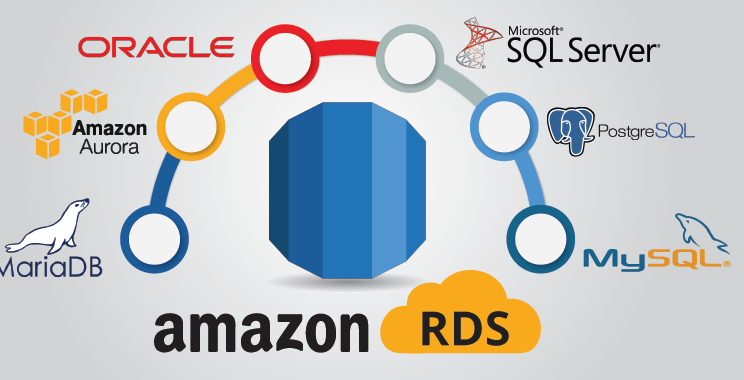
\includegraphics[width=\textwidth]{rds.png}
    \caption{Relational Database Service}
    \label{fig:rds}
\end{figure}

\par The pricing of Amazon Relational Database Service is based on usage. There are no upfront or minimum fees. The cost is dependent on various parameters such as instance hours, the number of input and output transactions, storage capacity, size of backup storage, or amount of Internet data transfer. Different applications use different instance types. The database instance is a fundamental element of the Amazon RDS. A database engine works in each database instance with function parameters and specific properties that determine and control the properties of the databases. Database instances can be created, configured, and deleted using the AWS CLI, AWS management console, or RDS API. Computing and storage and capacity, database engine, and other parameters such as backup, version and update settings, or master user access data must be specified for each database instance. Depending on the type of database engine the number of databases per instance varies for example, with Microsoft SQL Server, up to 100 databases are possible, Oracle allows one database per instance, MySQL, MariaDB, Amazon Aurora, and PostgreSQL have no software limitations on the maximum number of databases \cite{35}.

\par Security of Amazon RDS and the stored or transmitted data is implemented at various levels. AWS IAM controls which application or which user has access to which database resources and functions. Depending on the requirements, groups and users are created and specific access rights are assigned. Database instances are in a protected Amazon Virtual Private Cloud (VPC). VPC security groups control the access that traffic has in and out of a DB instance. By default, network access is turned off for a DB instance. Users can specify rules in a security group that allows access from an IP address range, port, or security group. After rules are configured, the same rules apply to all DB instances that are associated with that security group. It is possible to specify up to 20 rules in a security group. VPC security groups define which devices or instances can connect to a database instance. The connections are encrypted and secured using Transport Layer Security (TLS) / Secure Sockets Layer (SSL) or IPsec VPNs. Amazon RDS firewall settings control network access. Database data at rest can be encrypted and database events can be logged \cite{71}.

        {\textbf{Features of RDS Instances}
\begin{itemize}
    \item \textbf{Amazon RDS Resources Encryption:} Data that is encrypted includes the underlying storage for DB instances, its automated backups, snapshots, and read replicas. Amazon RDS encrypted DB instances use the industry standard AES-256 encryption algorithm to encrypt the data on the server that hosts the Amazon RDS DB instances. After enabling data encryption, Amazon RDS handles authentication of access and decryption of the data transparently with a minimal impact on performance. The database client doesn’t need any modification to use encryption \cite{35}.
\end{itemize}
\begin{itemize}
    \item \textbf{Automatic backups:} Amazon RDS provisions creation and saving automatic backups of RDS DB instance.
    It
    provides users the capability choose a retention period and restore databases to any time during that period.
    Users can also take snapshots of instances manually and these snapshots remains until manually deleted \cite{71}.
\end{itemize}
\begin{itemize}
    \item \textbf{Replication:} Amazon RDS uses the MariaDB, Microsoft SQL Server, MySQL, Oracle, and PostgreSQL DB engines' built-in replication functionality to create a special type of DB instance called a read replica from a source DB instance.\         It is a read-only copy
    of the
    actual database instance used by the application.\         It is possible to enable automatic fail over across availability
    zones with synchronous data replication and through RDS Multi-AZ deployment.
    Figure \ref{fig:readreplicasworking} provides a pictorial view of the working of read replica \cite{35}.
\end{itemize}
\begin{figure}
    \centering
    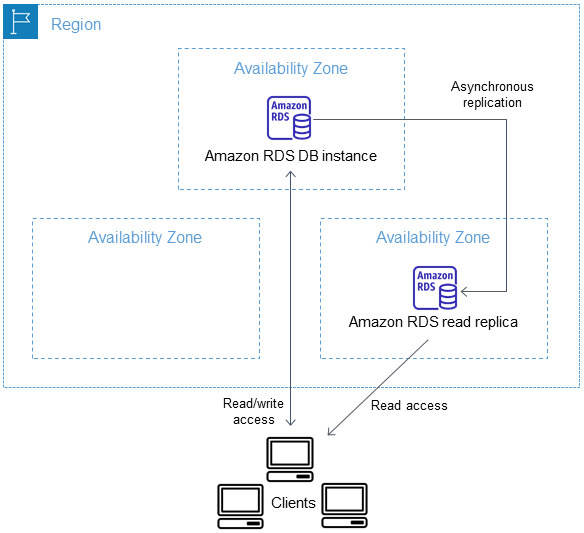
\includegraphics[width=\textwidth]{readreplicasworking.png}
    \caption{AWS RDS DB Instance Replication}
    \label{fig:readreplicasworking}
\end{figure}
\begin{itemize}
    \item \textbf{Performance metrics and monitoring:} Amazon provides CloudWatch service that enables managed
    monitoring.
    Amazon CloudWatch make it possible for the users to view capacity and I/O metrics \cite{35}.
\end{itemize}



\textbf{Amazon Simple Storage Service (S3)}

\par Amazon Simple Storage Service (Amazon S3) is an object storage service that offers industry-leading scalability, security, performance and data availability. Amazon S3 enables backup and archiving of data and applications in AWS. It can store any type of object, which allows uses like storage for Internet applications, data archives, backups, disaster recovery, hybrid cloud storage, IoT devices, and data lakes for analytics \cite{36}.

\par Storing, organizing, and retrieving data in Amazon S3 primarily focuses on two key components: objects and buckets that work together to create the storage system. The Amazon S3 object storage data model is a flat structure. A bucket is created and the bucket stores objects. There is no real hierarchy of sub buckets or subfolders but a logical hierarchy can be inferred using key name prefixes and delimiters. The objects are data files which include photos, documents, and videos. Each object in the S3 environment is identified by a unique key that differentiates it from other objects. The buckets serve as the fundamental storage containers for objects. While creating the bucket AWS provides users the ability to choose the AWS region. Even though a bucket is associated with a specified region, the name of the bucket acts as a global identifier, thus the name of the bucket must be unique among all the buckets across the world. The figure \ref{fig:s3} show Amazon S3, buckets and objects \cite{37}.

\par Amazon S3 offers features to organize and manage data to operate cost-effectively, support specific use cases,
increase security, and meet compliance requirements. With S3 Versioning, it is possible to keep multiple variants of an object in the same bucket. S3 Versioning helps to preserve, retrieve, and restore every version of every object stored in the buckets. Upon enabling S3 versioning in a bucket, Amazon S3 generates a unique version ID for each object added to the bucket. Objects that already existed in the bucket at the time versioning is enabled, such objects get assigned with a version ID of \textit{null}. If an object is modified, such as \textit{CopyObject} and \textit{PutObject}, the new objects get a unique version ID \cite{72}.

\begin{figure}
    \centering
    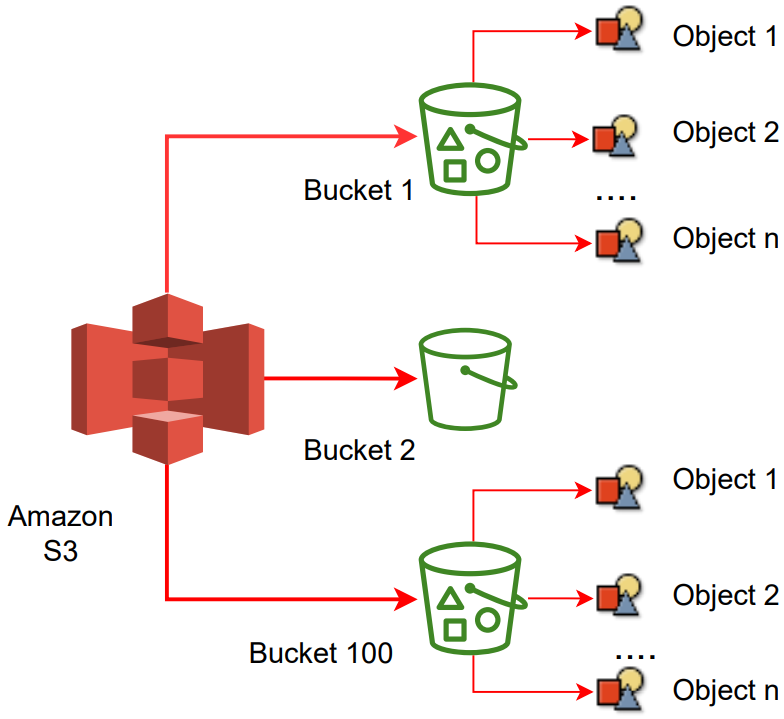
\includegraphics[width=\textwidth]{s3.png}
    \caption{Amazon Simple Storage Service}
    \label{fig:s3}
\end{figure}
\par Access to S3 objects is managed using the Identity and access management service (IAM), bucket policies, S3 access points, and Access Control Lists (ACLs). With the Identity and access management service (IAM), it is possible to manage the access on the user or group level, it is also possible to delegate permissions to the S3 bucket to other AWS customer accounts. A resource-based AWS Identity and Access Management (IAM) policy called a bucket policy is used to grant access permissions to the bucket and the objects. Only the bucket owner can associate a policy with a bucket. Bucket policies use JSON-based access policy language. The bucket policies can be used to add or deny permissions for the objects in a bucket. The permissions attached to the bucket apply to all the objects in the bucket. Bucket policies allow or deny requests based on the elements in the policy, this includes the requester, S3 actions, resources, and aspects or conditions of the request, for example, request an IP address. Amazon S3 Access Points describe how data can be accessed using that endpoint. Access Points are attached to buckets that is used to perform S3 object operations, such as \textit{GetObject} and \textit{PutObject}. Each S3 access point has its own access point policy. Access control lists (ACLs) grants read and write permissions to authorized users for individual buckets and objects. Each bucket and object have an ACL attached to it as a sub resource. The ACL defines which AWS groups or accounts are granted access and the type of access to which the access is granted. Amazon S3 Block Public Access feature provides settings for buckets, access points, and accounts to help you manage public access to Amazon S3 resources. By default, public access is not allowed on access points, new buckets, and objects, however, users can modify the access point policies, bucket policies, or object-related permissions to allow public access \cite{36}.

\par S3 Block Public Access provides four settings. It is possible to apply these settings in any combination to
individual buckets, access points, or entire AWS accounts. If the setting is applied to an account, it applies to all
buckets and access points that are owned by that account. Similarly, if the setting is applied to a bucket, it
applies to all access points associated with that bucket. Table \ref{tab:blockpublicaccesssettings} highlights
different settings for blocking public access \cite{23}.

\clearpage

\begin{longtable}{|p{5cm}|p{11.4cm}|}
    \hline
    \textbf{Name} & \textbf{Description} \\
    \hline
    \textit{BlockPublicAcls} & When BlockPublicAcls is set to TRUE the following behavior are seen:
    \begin{itemize}
        \item If the specified access control list (ACL) is public, PUT Bucket acl and PUT Object acl calls fail.
    \end{itemize}

    \begin{itemize}
        \item If the request includes a public ACL, PUT Object calls fail.
    \end{itemize}

    \begin{itemize}
        \item If this setting is applied to an account, then PUT Bucket calls fail if the request includes a public ACL.
    \end{itemize}
    \par When BlockPublicAcls is set to TRUE, the above specified operations fail, however, existing policies and ACLs for buckets and objects are not modified. This setting enables protecting against public access while allowing to audit, refine, or otherwise alter the existing policies and ACLs for buckets and objects \cite{23}.
    \\
    \hline
    \textit{IgnorePublicAcls} & Setting IgnorePublicAcls to TRUE causes Amazon S3 to ignore all public ACLs on a bucket and any objects it contains. This enables to safely block public access granted by ACLs while still allowing PUT Object calls that include a public ACL. Enabling IgnorePublicAcls doesn't affect the persistence of any existing ACLs and doesn't prevent new public ACLs from being set \cite{23}.  \\
    \hline
    \textit{BlockPublicPolicy} & When BlockPublicPolicy is set to TRUE for a bucket, Amazon S3 rejects calls to PUT Bucket policy if the BlockPublicPolicy allows public access. When BlockPublicPolicy is set to TRUE for an access point, Amazon S3 rejects calls to PUT access point policy and PUT Bucket policy that are made through the access point if BlockPublicPolicy (for either the access point or the underlying bucket) is public \cite{23}.  \\
    \hline
    \textit{RestrictPublicBuckets} & Setting RestrictPublicBuckets to TRUE restricts access to an access point or bucket with a public policy to only AWS service principals and authorized users within the bucket owner's account.  RestrictPublicBuckets blocks all cross-account access to the access point or bucket (except by AWS service principals), while still allowing users within the account to manage the access point or bucket.

    Enabling RestrictPublicBuckets doesn't affect existing access point or bucket policies, except that Amazon S3 blocks public and cross-account access derived from any public access point or bucket policy, including non-public delegation to specific accounts \cite{23}.  \\
    \hline
    \caption{Block public access settings}
    \label{tab:blockpublicaccesssettings}
\end{longtable}




\textbf{Lambda:}
\par AWS Lambda is a serverless computing service that lets the users run code without provisioning or managing servers. Lambda runs the code on a highly available compute infrastructure and performs all the administrative tasks of the compute resources, including server and operating system maintenance, capacity provisioning and automatic scaling, code monitoring, and logging \cite{38}.

\par With Lambda, it is possible to run code for virtually any type of application or backend service by supplying the code in one of the languages that Lambda supports. The code is organized into Lambda functions. Lambda runs the function only when needed and scales automatically, from a few requests per day to thousands per second. Lambda can run functions in response to events from other AWS services or can be invoked using the Lambda API. Users pay only for the compute time that Lambda consumes, there is no charge when the code is not running \cite{27}.

\par Lambda is an ideal compute service for many application scenarios, as long as the user can run the application code using the Lambda standard runtime environment and within the resources that Lambda provides. When using Lambda, users are responsible only for their code. Lambda manages the compute fleet of resources that offers a balance of memory, CPU, network, and other resources to run the code. Because these resources are managed by Lambda, users cannot customize the operating system or login to compute instances on provided runtimes. Lambda performs administrative and operational activities on behalf of users, including managing capacity, monitoring, and logging the Lambda functions. AWS manages the entire infrastructure layer of AWS Lambda and thus saves user time on operational tasks. AWS Lambda provides a distinctive architectural property by enabling many instances of the same function, or of different functions from the same AWS account, to execute concurrently. This makes AWS Lambda a good fit for deploying highly scalable cloud computing solutions \cite{39}.

\par AWS Lambda invokes the function in an execution environment. The execution environment provides an isolated and secure runtime environment and manages the resources required to run the function. The execution environment also provides lifecycle support for the function's runtime and any external extensions associated with the function. The runtime of function and each external extension are processes that run within the execution environment \cite{27}.

\par The lifecycle of the execution environment includes the following phases:
\begin{itemize}
    \item \textbf{Init phase}: In the init phase, Lambda unfreezes or creates an execution environment with the configured
    resources, downloads the code for the function and all layers, initializes the runtime, initializes any
    extensions, and then runs the function’s initialization code \cite{27}.
\end{itemize}
\begin{itemize}
    \item \textbf{Invoke phase}: During this phase, Lambda invokes the function handler. After the function runs to
    completion, Lambda prepares to handle another function invocation \cite{27}.
\end{itemize}
\begin{itemize}
    \item \textbf{Shutdown phase}: The shutdown phase is triggered if the Lambda function does not receive any invocations
    for a period of time. In the shutdown phase, Lambda shuts down the runtime, alerts the extensions to let them
    stop cleanly, and then removes the environment. Lambda sends a Shutdown event to each extension, which tells the extension that the environment is about to be shut down \cite{27}.
\end{itemize}


\section{Security Framework}

\begin{figure}
    \centering
    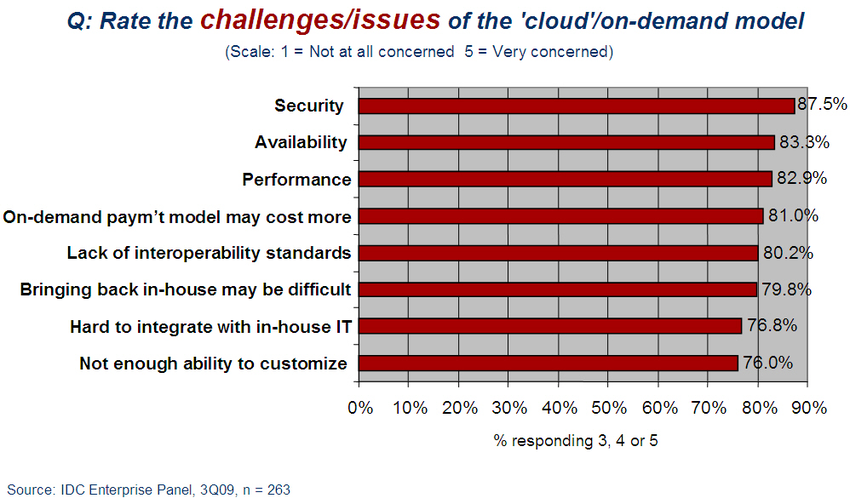
\includegraphics[width=\textwidth]{securitychallenges.png}
    \caption{Results of IDC ranking security challenges}
    \label{fig:securitychallenges}
\end{figure}

\par Cloud service providers (CSP) leverage virtualization technologies combined with self-service capabilities for computing resources via the Internet.
In these service provider environments, virtual machines from multiple organizations have to be co-located on the same physical server in order to maximize the efficiencies of virtualization.
CSP must learn from the managed service provider (MSP) and ensure that their customer’s data and applications are secure if CSP hopes to retain its customer base and competitiveness.
In a survey conducted by International Data Corporation
(IDC) as seen in the figure \ref{fig:securitychallenges},
of 263 IT executives and their line-of-business
colleagues to gauge their opinions and understand their companies’ use of IT cloud services, security is ranked first as the greatest issue or challenge of cloud computing \cite{79}.

\par In a world where digital transformation increases compliance burdens, understanding how to best secure on-premises, cloud, and hybrid IT stacks becomes more crucial than ever.
Information security management encompasses many areas from encryption and perimeter protection to application security and disaster recovery.
Security in IT is made more complex by compliance regulations, such as PCI, DSS, HIPAA, Sarbanes-Oxley, and global standards, such as GDPR. While most compliance experts and CEOs understand the value of cybersecurity measures, IT standards and security frameworks can make safeguarding organizations feel daunting.
Knowledge of standards, regulations, and frameworks is essential for all infosec and cybersecurity professionals \cite{80}.

\par A security framework is a compilation of state-mandated and international cybersecurity procedures and policies for maintaining and establishing security controls to protect critical infrastructure from cybersecurity risks.
These security frameworks are a blueprint for reducing vulnerabilities and managing risk by helping IT security professionals keep their organizations compliant and insulated from cyber threats.
The frameworks are used by Information security professionals to prioritize and define the tasks required to manage enterprise security.
It is possible for organizations to customize frameworks to solve specific information security problems, such as industry-specific requirements or different regulatory compliance goals \cite{80}.

\subsection{Prowler}

\par This research aims to introduce a framework called Prowler that can identify the security vulnerabilities or misconfigurations that exist in AWS accounts.
The thesis work focuses on the most popular AWS services,
IAM,
EC2, Lambda, S3, and RDS.
The introduced framework indicates to which security vulnerabilities the application is vulnerable and which security issues must be addressed to resolve the security vulnerability.
Prowler contains a set of controls, mapped against known security vulnerabilities, which can determine whether a given AWS cloud setup is vulnerable to these security vulnerabilities.
It aims to provide more in-depth security for AWS RDS,
EC2, IAM, S3, and Lambda resources and protects them
against security vulnerabilities.\\

\hfill \break
\par Prowler is an open-source AWS Security Best Practices Assessment, Hardening, Auditing, and Forensics Readiness command line tool.
Prowler scans the AWS account to check for potential security vulnerabilities, overly permissive Identity and Access Management (IAM) permissions, and best practice violations.
Using Prowler, it is possible to evaluate the AWS security specifically against the CIS AWS Foundations Benchmark and has more than 190 additional checks related to HIPAA, GDPR, PCI-DSS, ISO-27001, FFIEC, SOC2, and others \cite{75}.
Prowler provides more than 240 checks covering security best practices across all AWS regions and related to AWS services such as Amazon CloudFront, Amazon Redshift, Amazon ElasticCache, Amazon API Gateway, etc.
It helps organizations implement practices that ensure
having proper security measures in place and a secure
environment.
Prowler supports the generation of assessment reports in multiple formats such as JSON, CSV, HTML, JUnit, or JSON ASFF Security Hub.
The colorful or monochrome report enhances the user’s visibility.
Prowler also supports running a specific check or groups or creating your own.
When running the Prowler assessment, prowler supports
checking multiple AWS accounts in Parallel or
sequentially \cite{78}.\\
\hfill \break
\par Prowler is written in bash, and it uses AWS-CLI
underneath.
It works with multiple operating systems such
as macOS, Linux, or Windows with Cygwin or virtualization.
To use Prowler, though, an EC2 instance with the necessary security permissions can be provisioned, Fargate or any other container, CloudShell, Codebuild, and Cloud9.
Prowler can also be deployed directly in AWS using the AWS
CLI and other components such as Python pip,
detect-secrets, an open-source tool used to detect secrets by running scans, and jq , a flexible and lightweight command-line JSON processor already installed.
Detect-secrets is  \cite{78}.
\hfill \break
\begin{figure}
    \centering
    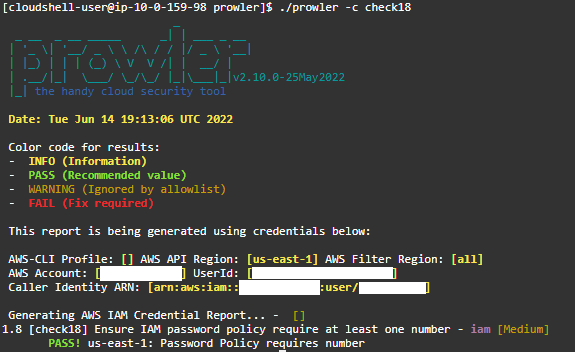
\includegraphics[width=\textwidth]{prowlercheckpass.png}
    \caption{Check execution in Prowler}
    \label{fig:prowlercheckexecution}
\end{figure}

\par After installing the required tools and packages
successfully, the AWS environment need be configured with
a valid Access Key and Region or by declaring the AWS
variables.
This can be done by running the command \textit{aws configure}.
In order to run all the Prowler checks, managed policies \textit{SecurityAudit} and \textit{ViewOnlyAccess} must be added to the user \cite{75}.



Prowler can then be installed directly by cloning the code for the source repository \cite{75} using the command \textit{git clone https://github.com/prowler-cloud/prowler} and does not require any additional setup afterward.
Once the source code is available, the assessment of security vulnerability using Prowler is performed by executing the command \textit{./prowler}.
Figure \ref{fig:prowlercheckexecution} shows the execution of the check using Prowler.
When the command is run, Prowler authenticates the configured environment variable.
Upon successful authentication, the checks are run over all the AWS regions.
To limit the assessment to a custom profile and region, the command \textit{./prowler -p custom-profile -r us-east-1} is used.
Prowler also enables assessing a single security vulnerability by running the command \textit{./prowler -c check78}.
The check78 is a check id, this check ensures there are no Public Accessible RDS instances (verifies publicly accessible RDS instances).
Table \ref{tab:prowlerextra} shows the execution result of the assessment performed using Prowler \cite{75}.
\begin{table}[h!]
    \begin{center}
        \caption{Prowler check execution result}
        \label{tab:prowlerextra}
        \begin{tabular}{|p{1.4cm}|p{1.7cm}|p{1.5cm}|p{4.0cm}|p{5.0cm}|}
            \hline
            \textbf{Result} & \textbf{Severity} & \textbf{CheckID} & \textbf{Check Title} & \textbf{Check Output}\\
            \hline
            Pass & Critical & 7.8 & [extra78] Ensure there are no Public Accessible RDS instances &
            No Publicly Accessible RDS instances found\\
            \hline
        \end{tabular}
    \end{center}
\end{table}

\par If the user wants to save the assessment report for later analysis, Prowler enables saving the result in different formats such as CSV, JSON, Html, etc.
This is achieved by using the command \textit{./prowler -M csv}\cite{75}.

\begin{figure}
    \centering
    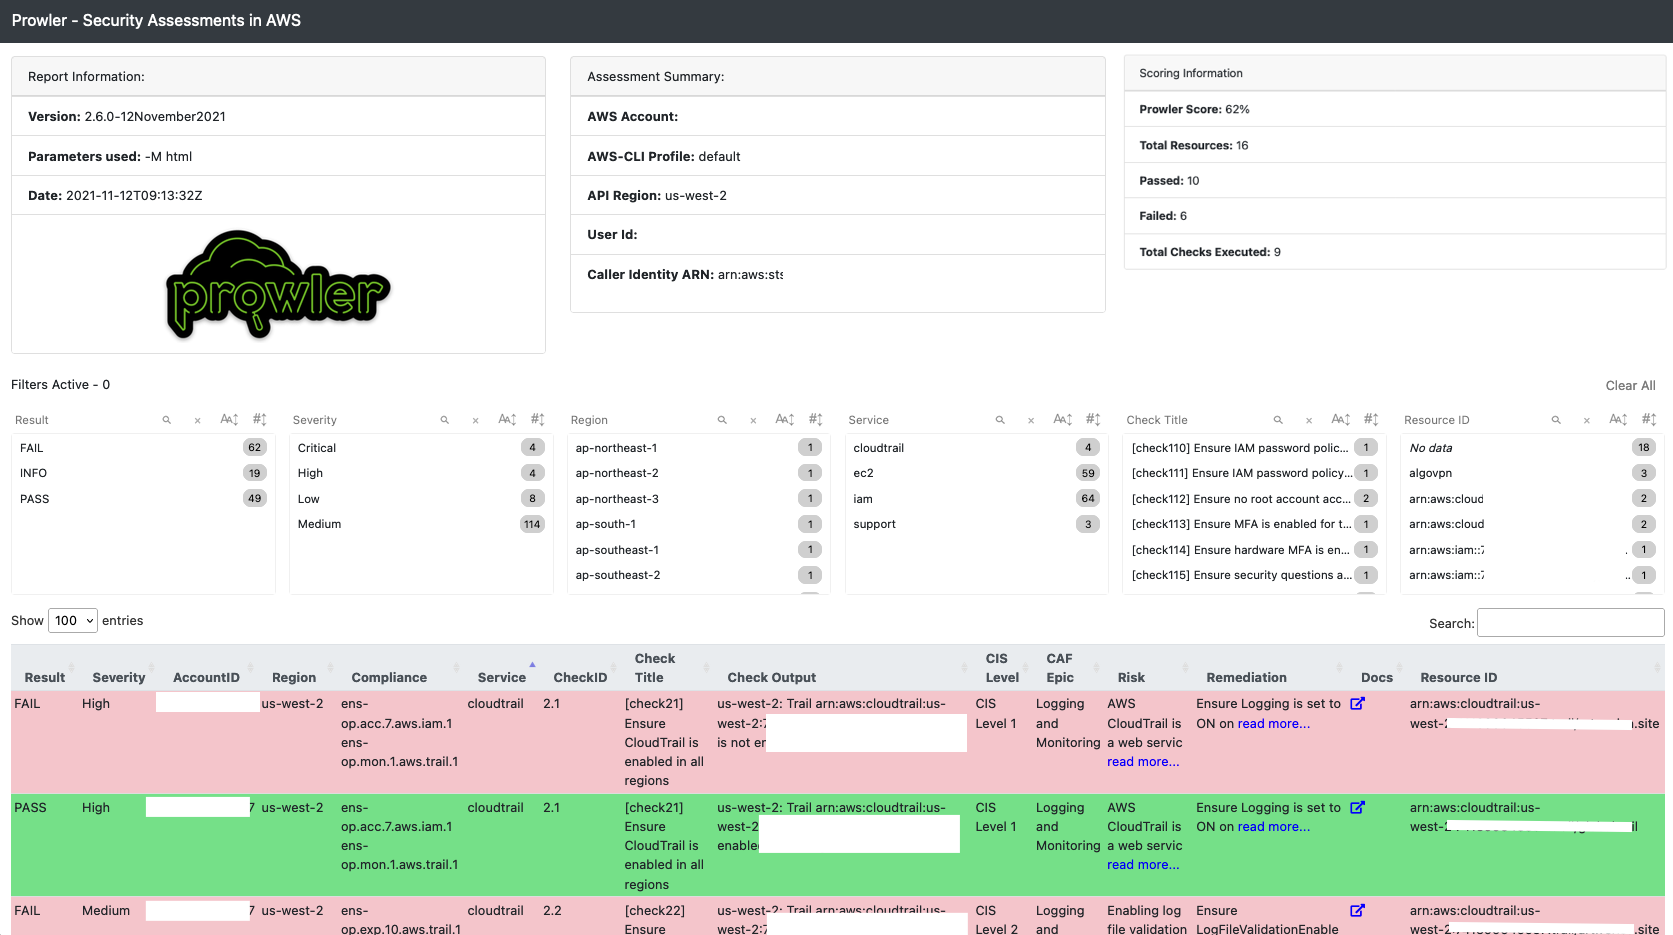
\includegraphics[width=\textwidth]{prowlerassessmentreport.png}
    \caption{Assessment report in Prowler}
    \label{fig:assessmentreport}
\end{figure}

The figure \ref{fig:assessmentreport} shows the
assessment report generated after the assessment of AWS
account using Prowler.